\hypertarget{phonefirewall__administration_8c}{
\section{phonefirewall\_\-administration.c File Reference}
\label{phonefirewall__administration_8c}\index{phonefirewall\_\-administration.c@{phonefirewall\_\-administration.c}}
}
{\tt \#include $<$stdio.h$>$}\par
{\tt \#include $<$stdlib.h$>$}\par
{\tt \#include $<$errno.h$>$}\par
{\tt \#include $<$string.h$>$}\par
{\tt \#include \char`\"{}libphonefirewall.h\char`\"{}}\par


Include dependency graph for phonefirewall\_\-administration.c:\nopagebreak
\begin{figure}[H]
\begin{center}
\leavevmode
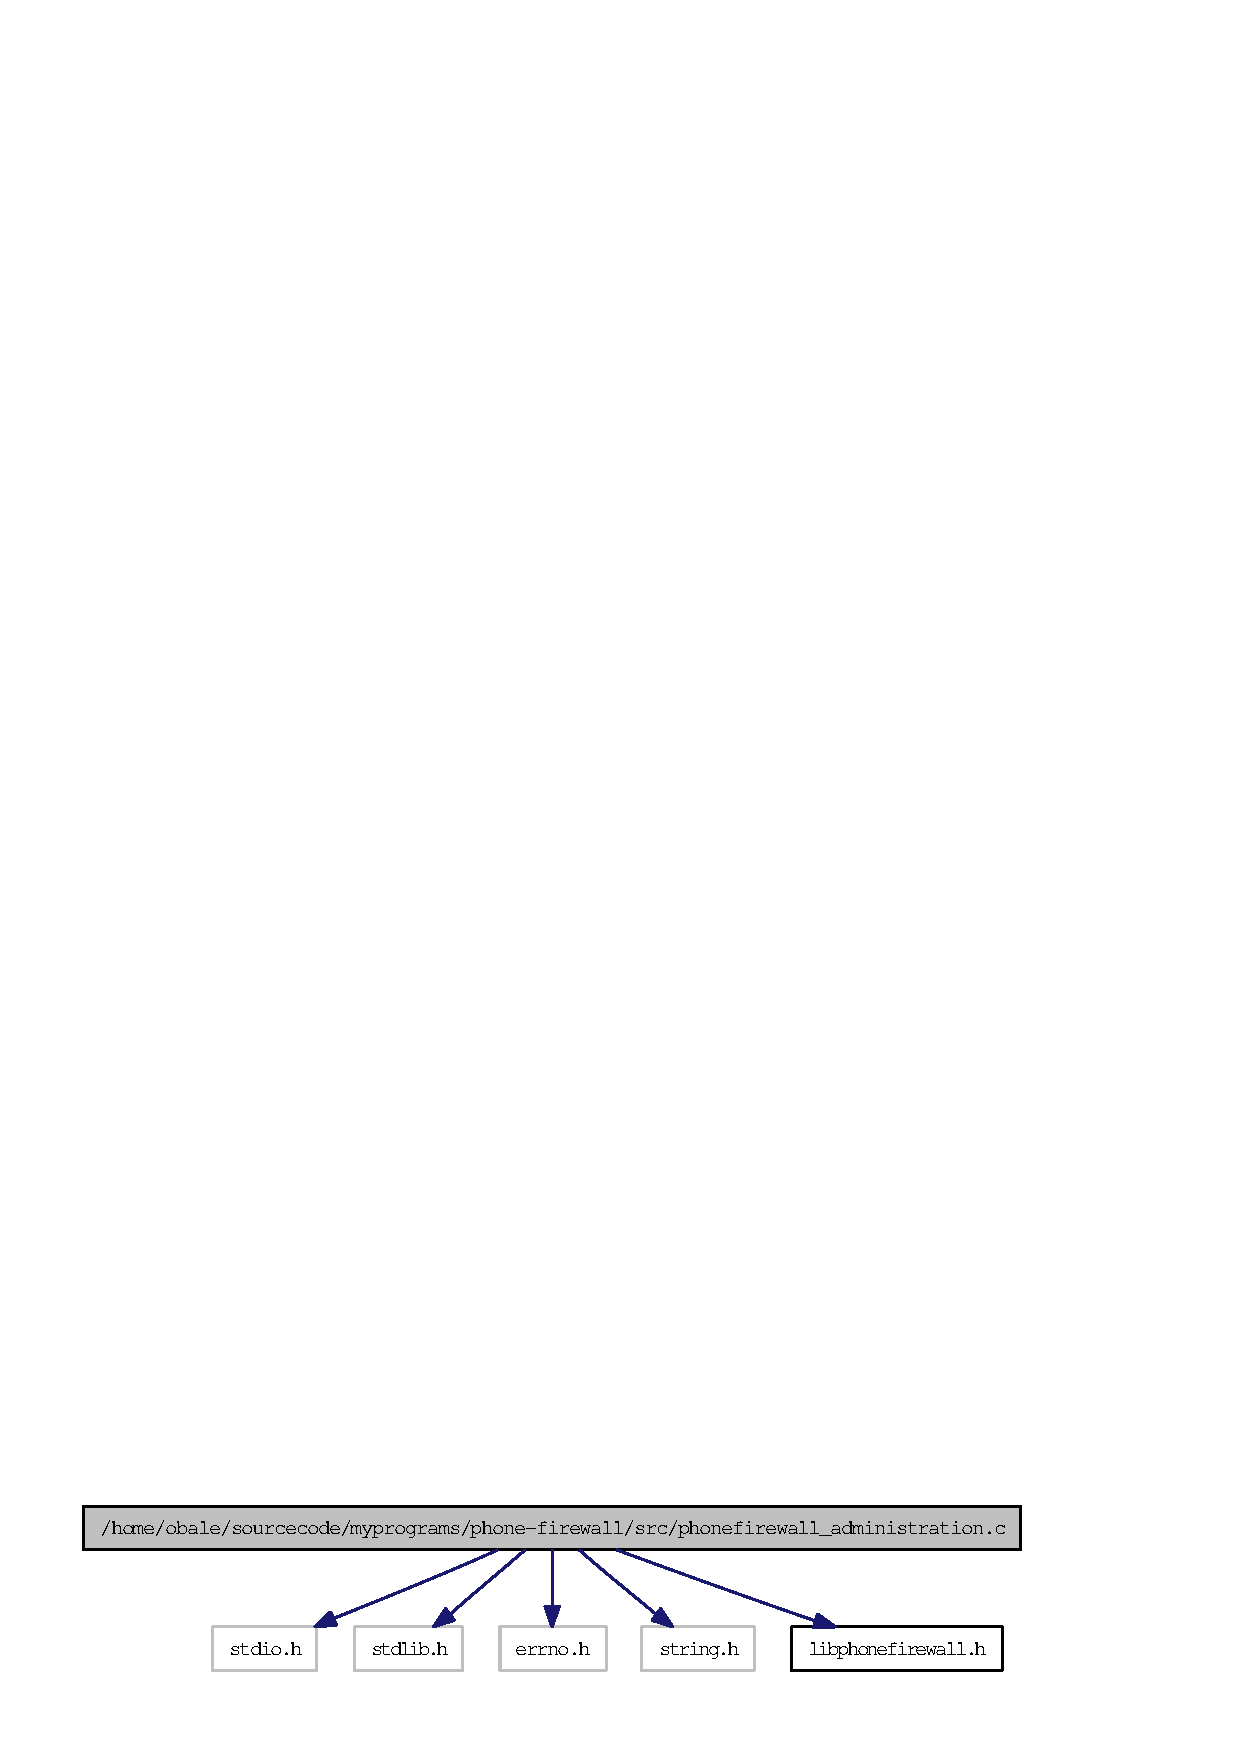
\includegraphics[width=211pt]{phonefirewall__administration_8c__incl}
\end{center}
\end{figure}
\subsection*{Defines}
\begin{CompactItemize}
\item 
\#define \hyperlink{phonefirewall__administration_8c_c0120f27d973f4ea90962305431fedce}{BLACKLIST\_\-PREFIX}~\char`\"{}db/blacklist\_\-\char`\"{}
\item 
\#define \hyperlink{phonefirewall__administration_8c_b5b8614b1e4d5e316cc4a8102ce9636c}{WHITELIST\_\-PREFIX}~\char`\"{}db/whitelist\_\-\char`\"{}
\item 
\#define \hyperlink{phonefirewall__administration_8c_03bc2a42c1399400ae0d103f5ada724c}{FILENAME\_\-SIZE}~256
\end{CompactItemize}
\subsection*{Functions}
\begin{CompactItemize}
\item 
int \hyperlink{phonefirewall__administration_8c_d42187af304bf25d98f7f7f76853c6f7}{set\_\-filename} (char $\ast$prefix, int country\_\-code, int area\_\-code)
\item 
int \hyperlink{phonefirewall__administration_8c_36847ed3459e2a89038772ece42a017d}{add\_\-blacklist\_\-entry} (int country\_\-code, int area\_\-code, unsigned long long number, char $\ast$name, char $\ast$reason, int priority)
\item 
int \hyperlink{phonefirewall__administration_8c_eec16cb88eb546b1a2490e6716d75f8b}{add\_\-whitelist\_\-entry} (int country\_\-code, int area\_\-code, unsigned long long number, char $\ast$name, char $\ast$reason, int priority)
\item 
int \hyperlink{phonefirewall__administration_8c_e6c567f38aaa0eaa9db3eb13e32cdbbd}{rm\_\-blacklist\_\-entry} (unsigned long long number)
\item 
int \hyperlink{phonefirewall__administration_8c_e8a4ee30cf26b05a55680dc3a972f1a4}{rm\_\-whitelist\_\-entry} (unsigned long long number)
\item 
char $\ast$ \hyperlink{phonefirewall__administration_8c_651cdd0245f20256305b40f13bb9df2d}{check\_\-blacklist\_\-entry} (int country\_\-code, int area\_\-code, unsigned long long number, int priority)
\item 
char $\ast$ \hyperlink{phonefirewall__administration_8c_032c45d6c7830492ddeaa8cabfc845c3}{check\_\-whitelist\_\-entry} (int country\_\-code, int area\_\-code, unsigned long long number, int priority)
\end{CompactItemize}
\subsection*{Variables}
\begin{CompactItemize}
\item 
static char $\ast$ \hyperlink{phonefirewall__administration_8c_6c7d3710dd8e86998206dad075d6fc27}{DELIM} = \char`\"{}::\char`\"{}
\item 
char \hyperlink{phonefirewall__administration_8c_89707f7a91e271cac7f8e4e2a0be0006}{filename} \mbox{[}FILENAME\_\-SIZE\mbox{]}
\end{CompactItemize}


\subsection{Define Documentation}
\hypertarget{phonefirewall__administration_8c_c0120f27d973f4ea90962305431fedce}{
\index{phonefirewall\_\-administration.c@{phonefirewall\_\-administration.c}!BLACKLIST\_\-PREFIX@{BLACKLIST\_\-PREFIX}}
\index{BLACKLIST\_\-PREFIX@{BLACKLIST\_\-PREFIX}!phonefirewall_administration.c@{phonefirewall\_\-administration.c}}
\subsubsection{\setlength{\rightskip}{0pt plus 5cm}\#define BLACKLIST\_\-PREFIX~\char`\"{}db/blacklist\_\-\char`\"{}}}
\label{phonefirewall__administration_8c_c0120f27d973f4ea90962305431fedce}




Definition at line 26 of file phonefirewall\_\-administration.c.

Referenced by add\_\-blacklist\_\-entry(), and check\_\-blacklist\_\-entry().\hypertarget{phonefirewall__administration_8c_03bc2a42c1399400ae0d103f5ada724c}{
\index{phonefirewall\_\-administration.c@{phonefirewall\_\-administration.c}!FILENAME\_\-SIZE@{FILENAME\_\-SIZE}}
\index{FILENAME\_\-SIZE@{FILENAME\_\-SIZE}!phonefirewall_administration.c@{phonefirewall\_\-administration.c}}
\subsubsection{\setlength{\rightskip}{0pt plus 5cm}\#define FILENAME\_\-SIZE~256}}
\label{phonefirewall__administration_8c_03bc2a42c1399400ae0d103f5ada724c}




Definition at line 28 of file phonefirewall\_\-administration.c.\hypertarget{phonefirewall__administration_8c_b5b8614b1e4d5e316cc4a8102ce9636c}{
\index{phonefirewall\_\-administration.c@{phonefirewall\_\-administration.c}!WHITELIST\_\-PREFIX@{WHITELIST\_\-PREFIX}}
\index{WHITELIST\_\-PREFIX@{WHITELIST\_\-PREFIX}!phonefirewall_administration.c@{phonefirewall\_\-administration.c}}
\subsubsection{\setlength{\rightskip}{0pt plus 5cm}\#define WHITELIST\_\-PREFIX~\char`\"{}db/whitelist\_\-\char`\"{}}}
\label{phonefirewall__administration_8c_b5b8614b1e4d5e316cc4a8102ce9636c}




Definition at line 27 of file phonefirewall\_\-administration.c.

Referenced by add\_\-whitelist\_\-entry(), and check\_\-whitelist\_\-entry().

\subsection{Function Documentation}
\hypertarget{phonefirewall__administration_8c_36847ed3459e2a89038772ece42a017d}{
\index{phonefirewall\_\-administration.c@{phonefirewall\_\-administration.c}!add\_\-blacklist\_\-entry@{add\_\-blacklist\_\-entry}}
\index{add\_\-blacklist\_\-entry@{add\_\-blacklist\_\-entry}!phonefirewall_administration.c@{phonefirewall\_\-administration.c}}
\subsubsection{\setlength{\rightskip}{0pt plus 5cm}int add\_\-blacklist\_\-entry (int {\em country\_\-code}, int {\em area\_\-code}, unsigned long long {\em number}, char $\ast$ {\em name}, char $\ast$ {\em reason}, int {\em priority})}}
\label{phonefirewall__administration_8c_36847ed3459e2a89038772ece42a017d}


Add a number to the blacklist. The number will be blocked after that.

\begin{Desc}
\item[Parameters:]
\begin{description}
\item[{\em country\_\-code}]The country code (for example 39 for Italy, 43 for Austria, and so one) \item[{\em area\_\-code}]The area code which indicates your mobile operator. \item[{\em number}]The telephone number of the person. \item[{\em name}]The name of the person. \item[{\em reason}]Why you have blocked this person. \item[{\em priority}]Gives the entry a priority. 0 is standard. If the priority is higher the value will be also blocked/accepted if a higher priority is choosen.\end{description}
\end{Desc}
\begin{Desc}
\item[Returns:]If all goes well 0 (zero) otherwise an errno code. \end{Desc}


Definition at line 40 of file phonefirewall\_\-administration.c.

References BLACKLIST\_\-PREFIX, DELIM, filename, and set\_\-filename().

Here is the call graph for this function:\nopagebreak
\begin{figure}[H]
\begin{center}
\leavevmode
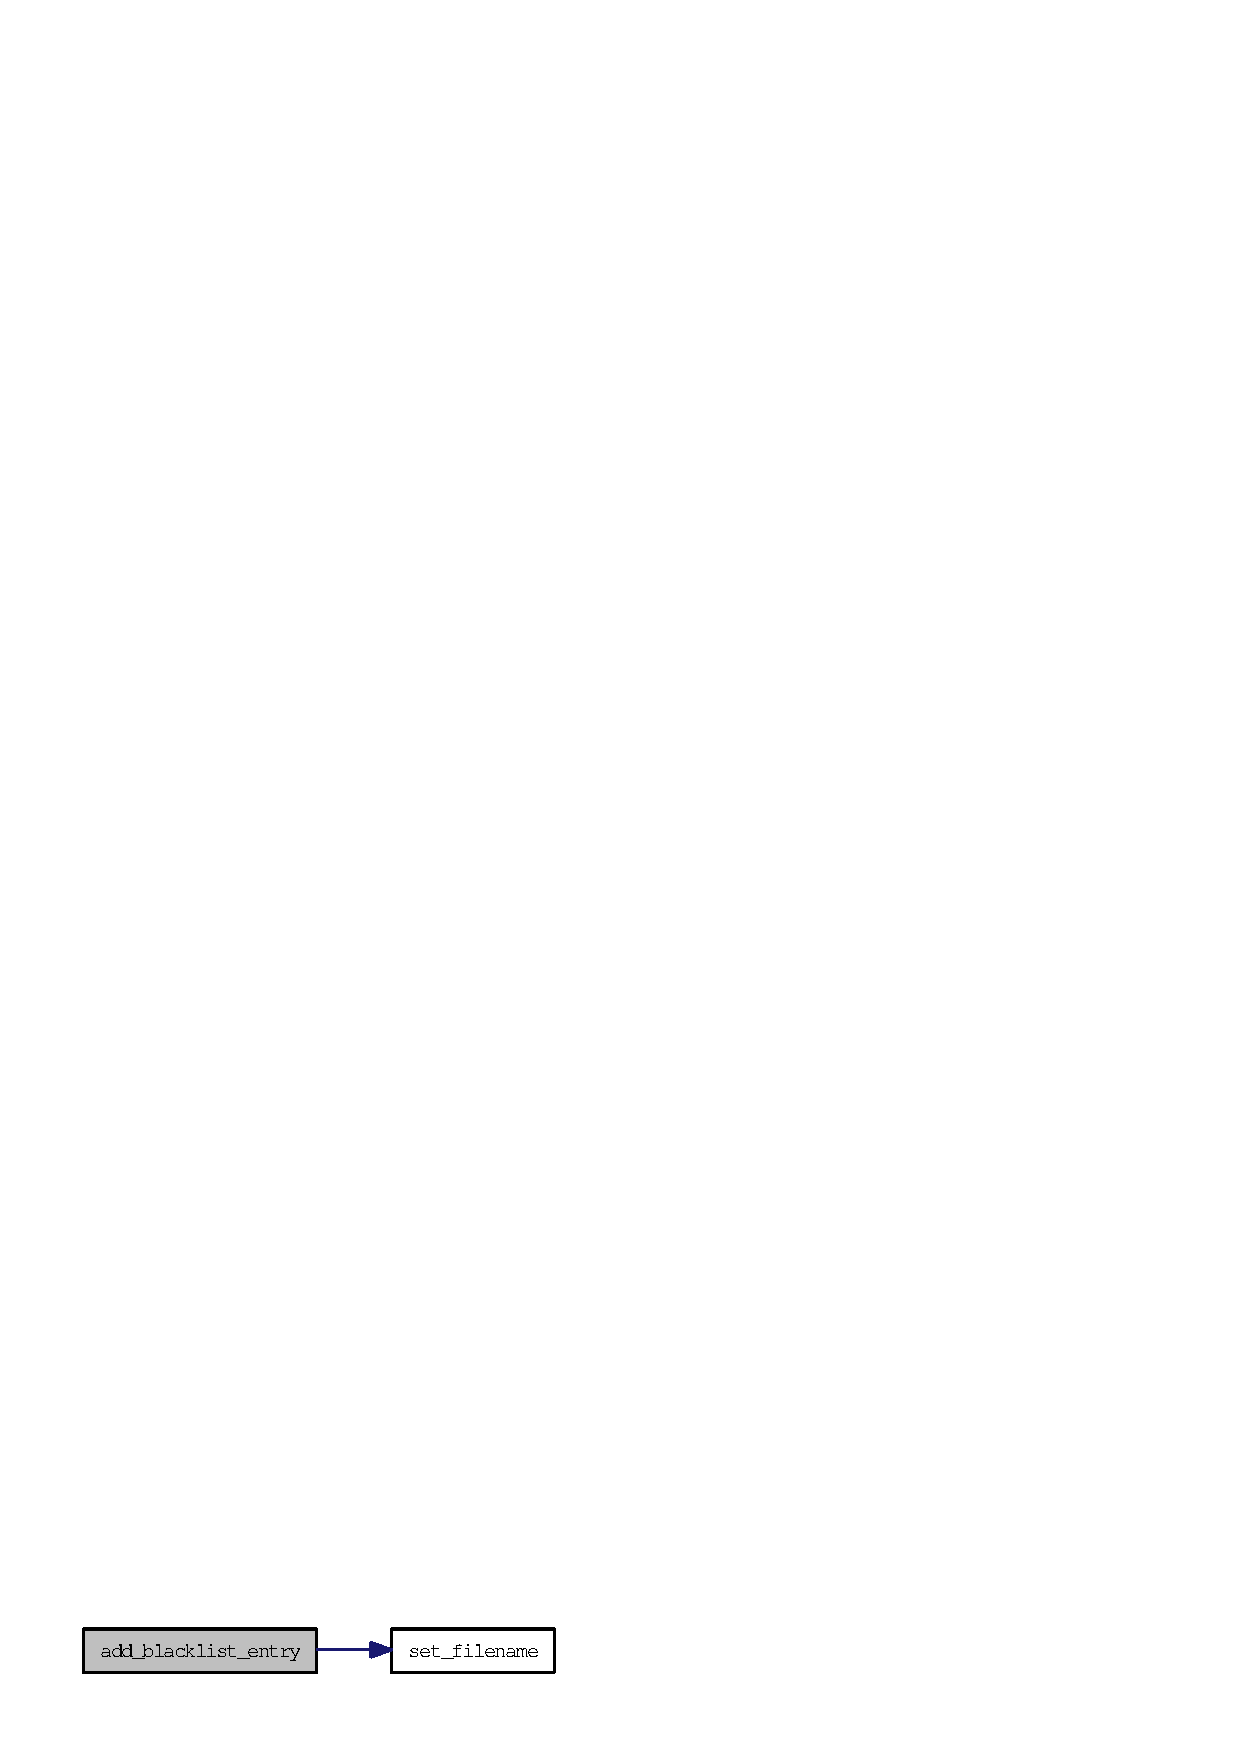
\includegraphics[width=135pt]{phonefirewall__administration_8c_36847ed3459e2a89038772ece42a017d_cgraph}
\end{center}
\end{figure}
\hypertarget{phonefirewall__administration_8c_eec16cb88eb546b1a2490e6716d75f8b}{
\index{phonefirewall\_\-administration.c@{phonefirewall\_\-administration.c}!add\_\-whitelist\_\-entry@{add\_\-whitelist\_\-entry}}
\index{add\_\-whitelist\_\-entry@{add\_\-whitelist\_\-entry}!phonefirewall_administration.c@{phonefirewall\_\-administration.c}}
\subsubsection{\setlength{\rightskip}{0pt plus 5cm}int add\_\-whitelist\_\-entry (int {\em country\_\-code}, int {\em area\_\-code}, unsigned long long {\em number}, char $\ast$ {\em name}, char $\ast$ {\em reason}, int {\em priority})}}
\label{phonefirewall__administration_8c_eec16cb88eb546b1a2490e6716d75f8b}


Add a number to the whitelist. The number will be accepted after that.

\begin{Desc}
\item[Parameters:]
\begin{description}
\item[{\em country\_\-code}]The country code (for example 39 for Italy, 43 for Austria, and so one) \item[{\em area\_\-code}]The area code which indicates your mobile operator. \item[{\em number}]The telephone number of the person. \item[{\em name}]The name of the person. \item[{\em reason}]Why you have blocked this person. \item[{\em priority}]Gives the entry a priority. 0 is standard. If the priority is higher the value will be also blocked/accepted if a higher priority is choosen.\end{description}
\end{Desc}
\begin{Desc}
\item[Returns:]If all goes well 0 (zero) otherwise an errno code. \end{Desc}


Definition at line 53 of file phonefirewall\_\-administration.c.

References DELIM, filename, set\_\-filename(), and WHITELIST\_\-PREFIX.

Here is the call graph for this function:\nopagebreak
\begin{figure}[H]
\begin{center}
\leavevmode
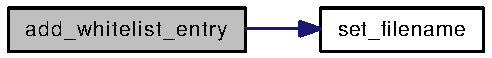
\includegraphics[width=136pt]{phonefirewall__administration_8c_eec16cb88eb546b1a2490e6716d75f8b_cgraph}
\end{center}
\end{figure}
\hypertarget{phonefirewall__administration_8c_651cdd0245f20256305b40f13bb9df2d}{
\index{phonefirewall\_\-administration.c@{phonefirewall\_\-administration.c}!check\_\-blacklist\_\-entry@{check\_\-blacklist\_\-entry}}
\index{check\_\-blacklist\_\-entry@{check\_\-blacklist\_\-entry}!phonefirewall_administration.c@{phonefirewall\_\-administration.c}}
\subsubsection{\setlength{\rightskip}{0pt plus 5cm}char$\ast$ check\_\-blacklist\_\-entry (int {\em country\_\-code}, int {\em area\_\-code}, unsigned long long {\em number}, int {\em priority})}}
\label{phonefirewall__administration_8c_651cdd0245f20256305b40f13bb9df2d}


Checks if a number is on the blacklist.

\begin{Desc}
\item[Parameters:]
\begin{description}
\item[{\em country\_\-code}]The country code (for example 39 for Italy, 43 for Austria, and so one) \item[{\em area\_\-code}]The area code which indicates your mobile operator. \item[{\em number}]The telephone number of the person. \item[{\em priority}]Gives the entry a priority. 0 is standard. If the priority is higher the value will be also blocked/accepted if a higher priority is choosen.\end{description}
\end{Desc}
\begin{Desc}
\item[Returns:]If noting is found NULL, otherwise the number. \end{Desc}


Definition at line 74 of file phonefirewall\_\-administration.c.

References BLACKLIST\_\-PREFIX, DELIM, filename, MAX\_\-LINE\_\-LENGTH, and set\_\-filename().

Here is the call graph for this function:\nopagebreak
\begin{figure}[H]
\begin{center}
\leavevmode
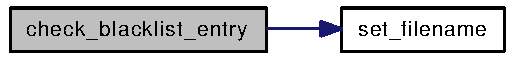
\includegraphics[width=141pt]{phonefirewall__administration_8c_651cdd0245f20256305b40f13bb9df2d_cgraph}
\end{center}
\end{figure}
\hypertarget{phonefirewall__administration_8c_032c45d6c7830492ddeaa8cabfc845c3}{
\index{phonefirewall\_\-administration.c@{phonefirewall\_\-administration.c}!check\_\-whitelist\_\-entry@{check\_\-whitelist\_\-entry}}
\index{check\_\-whitelist\_\-entry@{check\_\-whitelist\_\-entry}!phonefirewall_administration.c@{phonefirewall\_\-administration.c}}
\subsubsection{\setlength{\rightskip}{0pt plus 5cm}char$\ast$ check\_\-whitelist\_\-entry (int {\em country\_\-code}, int {\em area\_\-code}, unsigned long long {\em number}, int {\em priority})}}
\label{phonefirewall__administration_8c_032c45d6c7830492ddeaa8cabfc845c3}


Checks if a number is on the whitelist.

\begin{Desc}
\item[Parameters:]
\begin{description}
\item[{\em country\_\-code}]The country code (for example 39 for Italy, 43 for Austria, and so one) \item[{\em area\_\-code}]The area code which indicates your mobile operator. \item[{\em number}]The telephone number of the person. \item[{\em priority}]Gives the entry a priority. 0 is standard. If the priority is higher the value will be also blocked/accepted if a higher priority is choosen.\end{description}
\end{Desc}
\begin{Desc}
\item[Returns:]If noting is found NULL, otherwise the number. \end{Desc}


Definition at line 105 of file phonefirewall\_\-administration.c.

References DELIM, filename, MAX\_\-LINE\_\-LENGTH, set\_\-filename(), and WHITELIST\_\-PREFIX.

Here is the call graph for this function:\nopagebreak
\begin{figure}[H]
\begin{center}
\leavevmode
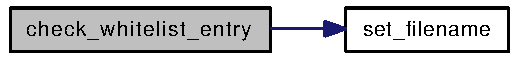
\includegraphics[width=142pt]{phonefirewall__administration_8c_032c45d6c7830492ddeaa8cabfc845c3_cgraph}
\end{center}
\end{figure}
\hypertarget{phonefirewall__administration_8c_e6c567f38aaa0eaa9db3eb13e32cdbbd}{
\index{phonefirewall\_\-administration.c@{phonefirewall\_\-administration.c}!rm\_\-blacklist\_\-entry@{rm\_\-blacklist\_\-entry}}
\index{rm\_\-blacklist\_\-entry@{rm\_\-blacklist\_\-entry}!phonefirewall_administration.c@{phonefirewall\_\-administration.c}}
\subsubsection{\setlength{\rightskip}{0pt plus 5cm}int rm\_\-blacklist\_\-entry (unsigned long long {\em number})}}
\label{phonefirewall__administration_8c_e6c567f38aaa0eaa9db3eb13e32cdbbd}


Removes a blocked number from the blacklist.

\begin{Desc}
\item[Parameters:]
\begin{description}
\item[{\em number}]The number which will be deleted.\end{description}
\end{Desc}
\begin{Desc}
\item[Returns:]If all goes right 0, otherwise an error code. \end{Desc}


Definition at line 66 of file phonefirewall\_\-administration.c.\hypertarget{phonefirewall__administration_8c_e8a4ee30cf26b05a55680dc3a972f1a4}{
\index{phonefirewall\_\-administration.c@{phonefirewall\_\-administration.c}!rm\_\-whitelist\_\-entry@{rm\_\-whitelist\_\-entry}}
\index{rm\_\-whitelist\_\-entry@{rm\_\-whitelist\_\-entry}!phonefirewall_administration.c@{phonefirewall\_\-administration.c}}
\subsubsection{\setlength{\rightskip}{0pt plus 5cm}int rm\_\-whitelist\_\-entry (unsigned long long {\em number})}}
\label{phonefirewall__administration_8c_e8a4ee30cf26b05a55680dc3a972f1a4}


Removes a accepted number from the whitelist.

\begin{Desc}
\item[Parameters:]
\begin{description}
\item[{\em number}]The number which will be deleted.\end{description}
\end{Desc}
\begin{Desc}
\item[Returns:]If all goes right 0, otherwise an error code. \end{Desc}


Definition at line 70 of file phonefirewall\_\-administration.c.\hypertarget{phonefirewall__administration_8c_d42187af304bf25d98f7f7f76853c6f7}{
\index{phonefirewall\_\-administration.c@{phonefirewall\_\-administration.c}!set\_\-filename@{set\_\-filename}}
\index{set\_\-filename@{set\_\-filename}!phonefirewall_administration.c@{phonefirewall\_\-administration.c}}
\subsubsection{\setlength{\rightskip}{0pt plus 5cm}int set\_\-filename (char $\ast$ {\em prefix}, int {\em country\_\-code}, int {\em area\_\-code})}}
\label{phonefirewall__administration_8c_d42187af304bf25d98f7f7f76853c6f7}




Definition at line 34 of file phonefirewall\_\-administration.c.

References filename.

Referenced by add\_\-blacklist\_\-entry(), add\_\-whitelist\_\-entry(), check\_\-blacklist\_\-entry(), and check\_\-whitelist\_\-entry().

Here is the caller graph for this function:\nopagebreak
\begin{figure}[H]
\begin{center}
\leavevmode
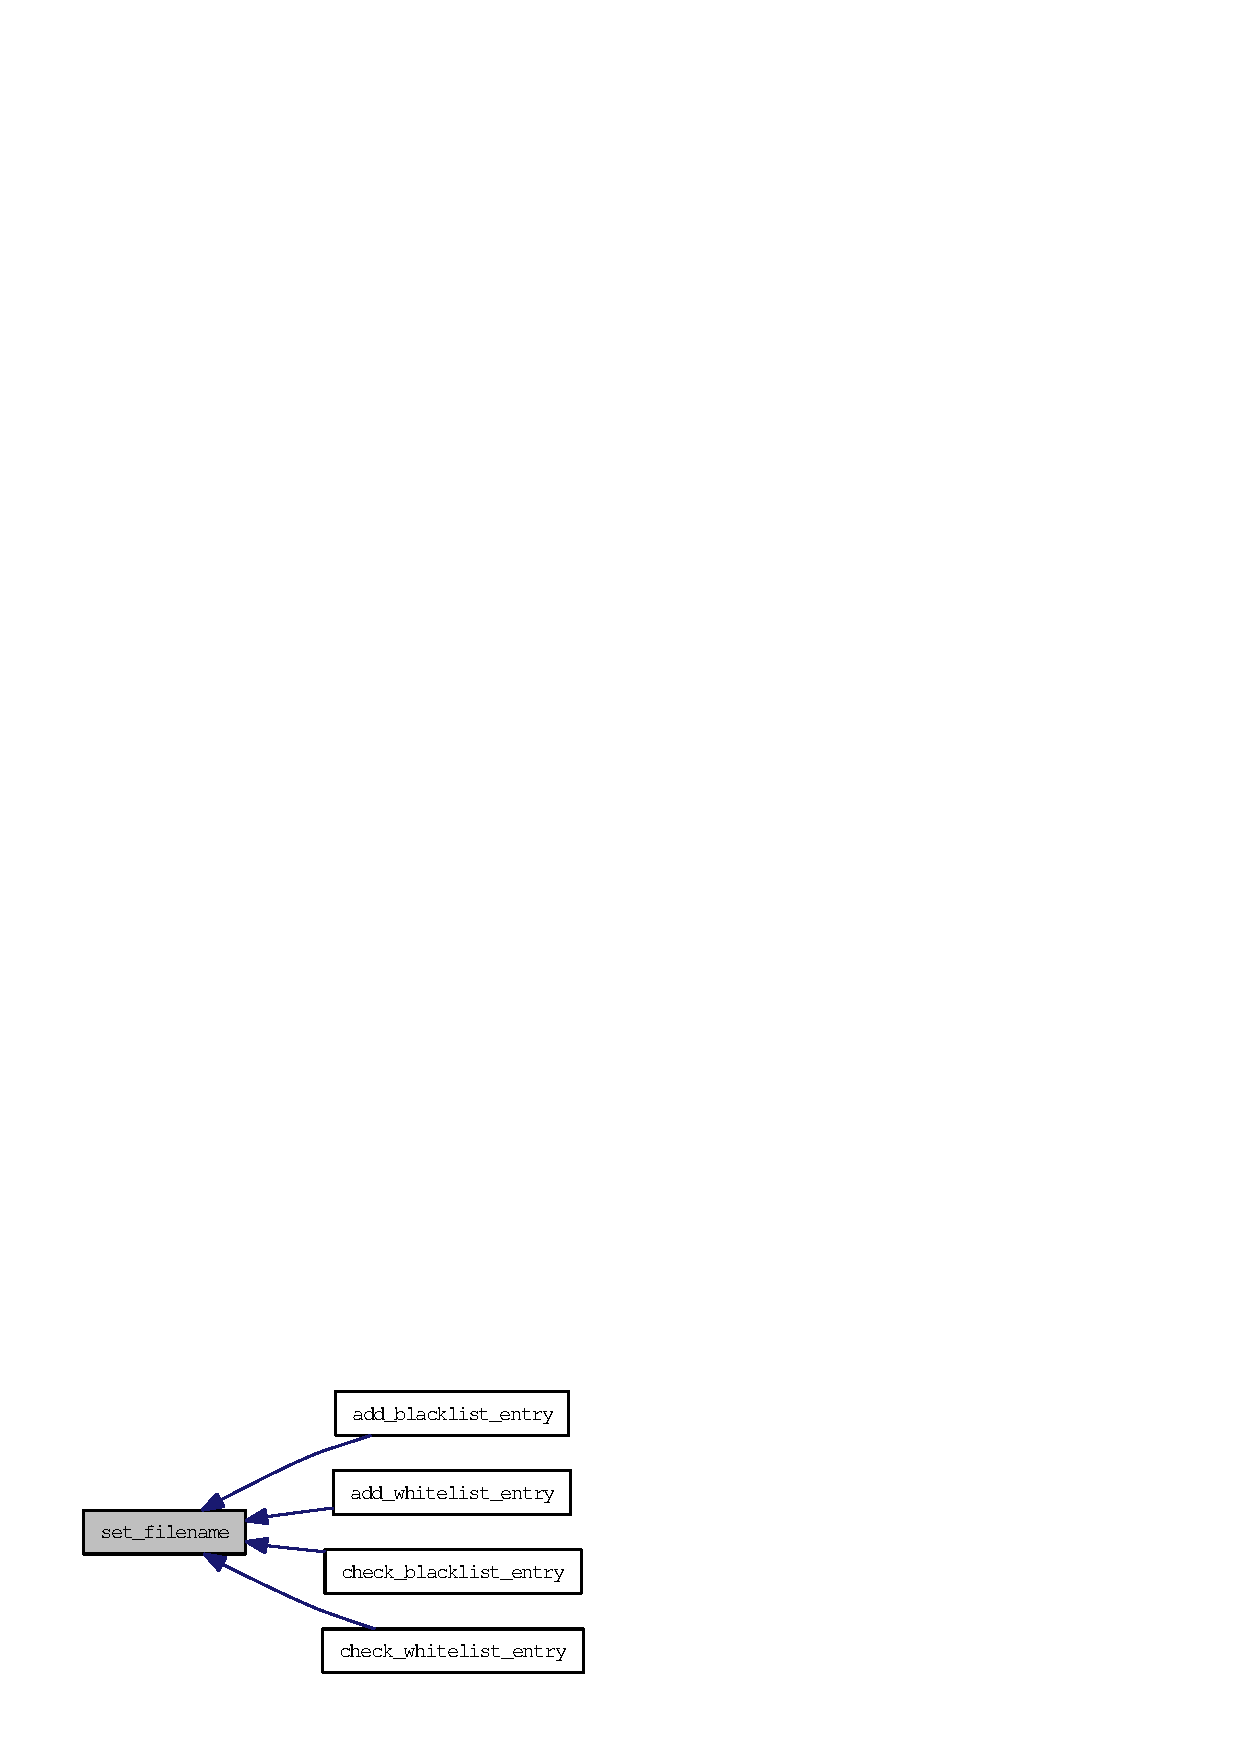
\includegraphics[width=142pt]{phonefirewall__administration_8c_d42187af304bf25d98f7f7f76853c6f7_icgraph}
\end{center}
\end{figure}


\subsection{Variable Documentation}
\hypertarget{phonefirewall__administration_8c_6c7d3710dd8e86998206dad075d6fc27}{
\index{phonefirewall\_\-administration.c@{phonefirewall\_\-administration.c}!DELIM@{DELIM}}
\index{DELIM@{DELIM}!phonefirewall_administration.c@{phonefirewall\_\-administration.c}}
\subsubsection{\setlength{\rightskip}{0pt plus 5cm}char$\ast$ {\bf DELIM} = \char`\"{}::\char`\"{}\hspace{0.3cm}{\tt  \mbox{[}static\mbox{]}}}}
\label{phonefirewall__administration_8c_6c7d3710dd8e86998206dad075d6fc27}




Definition at line 30 of file phonefirewall\_\-administration.c.

Referenced by add\_\-blacklist\_\-entry(), add\_\-whitelist\_\-entry(), check\_\-blacklist\_\-entry(), and check\_\-whitelist\_\-entry().\hypertarget{phonefirewall__administration_8c_89707f7a91e271cac7f8e4e2a0be0006}{
\index{phonefirewall\_\-administration.c@{phonefirewall\_\-administration.c}!filename@{filename}}
\index{filename@{filename}!phonefirewall_administration.c@{phonefirewall\_\-administration.c}}
\subsubsection{\setlength{\rightskip}{0pt plus 5cm}char {\bf filename}\mbox{[}FILENAME\_\-SIZE\mbox{]}}}
\label{phonefirewall__administration_8c_89707f7a91e271cac7f8e4e2a0be0006}




Definition at line 32 of file phonefirewall\_\-administration.c.

Referenced by add\_\-blacklist\_\-entry(), add\_\-whitelist\_\-entry(), check\_\-blacklist\_\-entry(), check\_\-whitelist\_\-entry(), and set\_\-filename().